\subsection{Распределение вычислительной нагрузки \\ с дроблением блоков сетки}

При использовании блочно-структурированной расчетной сетки\label{term:mesh_block_struct3} даже оптимальное решение задачи о распределении блоков по вычислиттелям суперкомпьютера не приводит к эффективному выполнению задачи.
При возрастании количества доступных вычислителей скорость работы задача упирается в обработку самого крупного блока.
Для достижения эффективного распределения вычислительной нагрузки требуется выполнять дробление отдельных крупных блоков.
В этом разделе рассмотрены алгоритмы дробления блоков блочно-структурированной расчетной сетки и описаны эксперименты по влиянию дробления блоков на эффективность проведения вычислений.

\subsubsection{Дробление блоков}

Одним из важнейших для распределения вычислительной нагрузки действий по управлению расчетной блочно-структурированной сеткой при выполнении вычислений на суперкомпьютере является дробление ее блоков \cite{Rybakov2016WithCut}.
Так как при запуске задач на суперкомпьютере постоянно возрастает степень параллельности (используется все больше параллельных процессов обработки блоков сетки), то для сохранения равномерности распределения блоков по вычислительным процессам требуется уметь измельчать блоки.
Блок сетки может быть разделен на два блока по любому из трех направлениий: $I$, $J$, $K$.

Кроме блоков сетка содержит другие объекты, которые требуют корректировки после разделения блока.
Сюда относятся интерфейсы, описывающие касание блоков друг друга.
На границе расчетной области граничные условия задаются с помощью специальных объектов, которые также должны быть разделены в случае пересечения их линией разреза блока.
Также должны быть по необходимости разделены области, описывающие начальные условия.
Каждыий из этих объектов имеет жесткую привязку к блоку, а значит после дробления может возникнуть
необходимость разделения этого объекта.

Граничные условия и области начальных условий обрабатываются наиболее просто и похожим образом.
Рассмотрим, например, граничные условия в двумерном случае (в координатах $IJ$).

\begin{figure}[ht]
\centering
\begin{tabular}{ll}
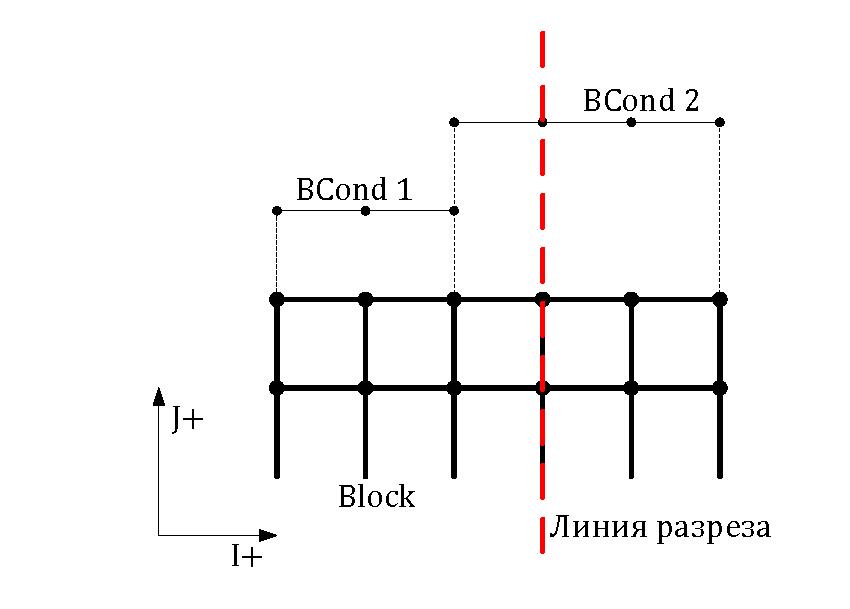
\includegraphics[width=0.45\textwidth]{./pics/text_2_withcut/cut-bcond.pdf}
&
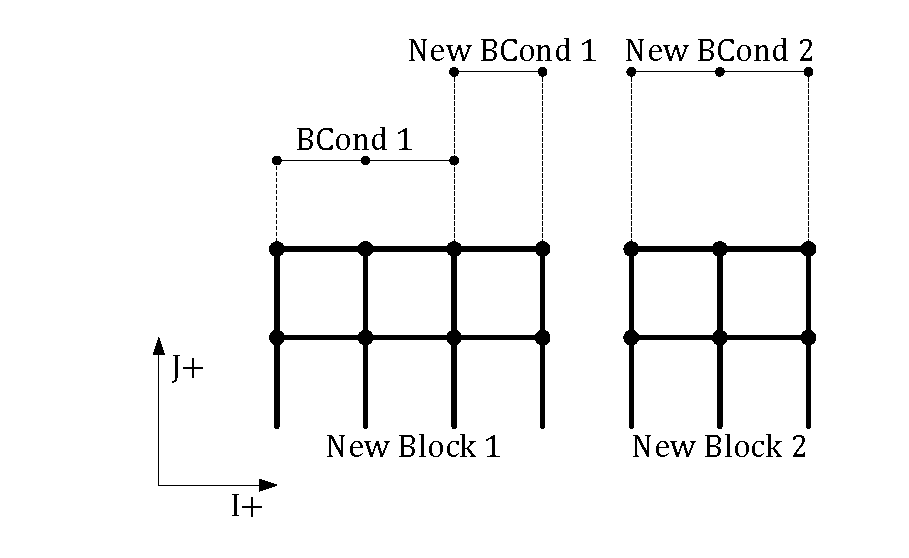
\includegraphics[width=0.45\textwidth]{./pics/text_2_withcut/cut-bcond2.pdf}
\end{tabular}
\singlespacing
\captionstyle{center}\caption{Дробление блока может спровоцировать дробление других объектов сетки.}
\label{fig:text_2_withcut_cut_bcond}
\end{figure}

Пусть блок Block должен быть разрезан по направлению $I+$ как показано на рис.~\ref{fig:text_2_withcut_cut_bcond} слева.
Пусть этот блок имеет граничные условия по направлению $J+$.
Тогда возможны два варианта.
Либо линия разреза не пересекает граничное условие, и тогда граничное условие целиком отходит одному из результирующих блоков (BCond 1).
Если же линия разреза проходит через граничное условие, то данное граничное условие также должно быть разделено, и его части отойдут двум результирующим блокам (рис.~\ref{fig:text_2_withcut_cut_bcond}, справа). Такая же ситуация может сложиться в отношении областей начальных условий.
В случае дробления интерфейсов могут быть более сложные ситуации дробления.

\subsubsection{Равномерное распределение блоков по вычислительным \\ процессам}

Для равномерного распределения блоков сетки по вычислительным процессам рассмотрим следующую задачу разделения множества весов на $m$ множеств.

Рассмотрим множество $X$ вещественных чисел $x_i \ge 0$ для $i \in N$, где $N = [1, n]$.
Рассмотрим также множество индексов $j \in M$, где $M = [1, m]$.
Будем говорить, что определено разбиение множества $X$ на $m$ множеств, если введена функция $\gamma(i): N \rightarrow M$.
Множество всех функций разбиения будем обозначать $\Gamma(N, M)$.
Веса результирующих множеств будем определять естественным образом для $j \in M$:
\begin{equation}
	X_j = \sum_{\substack{i \in N \\ \gamma(i) = j}}{x_i}
\end{equation}

Требуется найти такую функцию разбиения $\gamma \in \Gamma(N, M)$, чтобы минимизировать наиболее тяжелое из результирующих множеств $\max_{j \in M}{X_j}$.

Задача может быть расширена на случай распределения вычислительной нагрузки между вычислителями суперкомпьютера с разной производительностью.
При этом формулировка задачи меняется только в части приведения всех узлов к одному показателю с помощью весовых коэффициентов.

Коэффициентом приведения $\kappa(j)$ для $j \in M$ назовем такую положительную функцию $\kappa: M \rightarrow \mathbb{R}_{>0}$, что время выполнения нагрузки $\kappa(j)$ на узле $j$ не зависит от $j$.
Тогда в общем случае задача о равномерном разбиении множества весов на $m$ множеств с коэффициентами приведения $\kappa(j)$ для $j \in M$ формулируется следующим образом.
Требуется найти такую функцию разбиения $\gamma \in \Gamma(N, M)$, чтобы минимизировать наболее тяжелое из результирующих множеств с учетом коэффициентов приведения $\max_{j \in M}{ \frac{X_j}{\kappa(j)} }$.

Эта задача имеет практическое применение при распределении вычислительной нагрузки между вычислителями гетерогенного суперкомпьютера\label{term:cluster_getero2}.

Сформулированная задача является NP-полной, однако ее можно решить приближенно с помощью жадного алгоритма.
В жадном алгоритме будем последовательно обрабатывать все веса, начиная с наибольшего.
Каждый необработанный вес будем относить к наиболее легкому на текущий момент множеству весов.
Этот алгоритм является упрощенной версией алгоритма распределения вычислительной нагрузки между узлами гетерогенного вычислительного кластера, описанного в разделе \ref{sec:text_2_getero}.

Приведем оценку эффективности работы алгоритма.
Для удобства без ограничения общности будем считать, что изначальное множество весов упорядочено по убыванию.

Определим остаточный член $r_i$ для $i \in N$ по следующей формуле:
\begin{equation}
	r_i = \max{\left( x_i - \frac{1}{m} \sum_{p = i}^{n}{x_p}, 0 \right)}
\end{equation}

Тогда верно следующее утверждение

\begin{lemma}\label{lem:text_2_withcut_lem}
При использовании жадного алгоритма распределения весов между отдельными множествами отклонение наиболее тяжелого множества $\max_{j \in M}{X_j}$ от среднего значения веса множеств $\langle X \rangle$ не превышает максимальный остаточный член $r_i$, то есть
\begin{equation}
	\max_{j \in M}{X_j} - \langle X \rangle \le \max_{i \in N}{r_i}
\end{equation}
\end{lemma}
Пусть $X_k = \max_{j \in M}{X_j}$ -- наиболее тяжелое множество, а $x_t$ -- последний добавленный в него элемент.
Так как алгоритм является жадным, то до обработки веса $x_t$, $k$-е множество не превосходит по весу никакое другое множество, причем для любого $j \in M$ выполняется соотношение
\begin{equation}\label{lem:text_2_withcut_lem_single}
	X_k - x_t \le X_j - \chi_j,
\end{equation}	
	
где $\chi_j$ -- сумма весов, добавленных в $j$-е множество начиная с момента обработки веса $x_t$.
В частности, можно заметить, что $\chi_k = x_t$.

Почленно суммируя \eqref{lem:text_2_withcut_lem_single} по $j \in M$ получим соотношение
\begin{equation}
	m X_k - m x_t \le \sum_{j \in M}{X_j} - \sum_{p = t}^{n}{x_p},
\end{equation}

после деления которого на $m$ и переноса членов в нужные части неравенства, получим $X_k - \langle X \rangle \le r_t$ откуда следует утверждение леммы.
$\blacksquare$\\

Таким образом, для оценки эффективности описанного жадного алгоритма распределения весов по $m$ множествам достаточно проанализировать ряд остаточных членов, полученный из отсортированного массива распределяемых весов.

Задачу о равномерном распределении весов по результирующим множествам можно применить для равномерного распределения блоков блочно-структурированной расчетной сетки по вычислительным процессам суперкомпьютера в предположении, что все процессы равнозначны (не рассматривается случай гетерогенной системы).
В качестве веса блока нужно взять количество его ячеек.
Также заметим, что применительно к задаче распределения блоков расчетной сетки по вычислителям гомогенной системы оценка, полученная в лемме~\ref{lem:text_2_withcut_lem}, является оценкой показателя $D$ неравномерности распределения вычислительной нагрузки\label{term:decomp_neravn2}. 

Так как абсолютно равномерное распределение блоков по вычислительным процессам не всегда возможно, то нужно принять порог максимально допустимого отклонения количества ячеек одного процесса от среднего значения, при достижении которого распределение можно считать успешным.
Экспериментальным путем установлено, что порог максимального отклонения в 10\% является вполне достаточным для достижения эффективного распределения.
Если текущее распределение не удовлетворяет допустимому порогу отклонения количества ячеек процесса от среднего значения, то наиболее крупные блоки следует раздробить, после чего повторить оценку распределения.

\subsubsection{Результаты распределения блоков по процессам}

Рассмотренный алгоритм распределения вычислительной нагрузки блочно-структурированной сетки с дроблением блоков (применялось дробление наиболее крупных блоков пополам по наиболее протяженному направлению) между узлами гомогенной вычислительной системы был протестирован на различных расчетных сетках.
Ниже представлен результат тестирования на двух расчетных сетках.

Первая рассматриваемая сетка содержит 13 блоков, 80 интерфейсов, 148 граничных условий, 13 областей начальных условий и 5,75 млн ячеек, размер вычислительной окрестности равен 3.
Вторая рассматриваемая сетка содержит 300 блоков, 1796 интерфейсов, 1643 граничных условия, 300 областей начальных данных и 94,34 млн ячеек.
Размер вычислительной окрестности также равен 3.

Для этих сеток были проведены вычисления на 128 параллельных процессах.
Статистика распределения блоков по вычислительным процессам для двух различных вариантов: без использования дробления блоков и с использованием дроблений для достижения показателя неравномерности распределения распределения не более $D^{\%} = 10\%$ (см. рис.~\ref{fig:text_2_withcut_charts}).

\begin{figure}[ht]
\centering
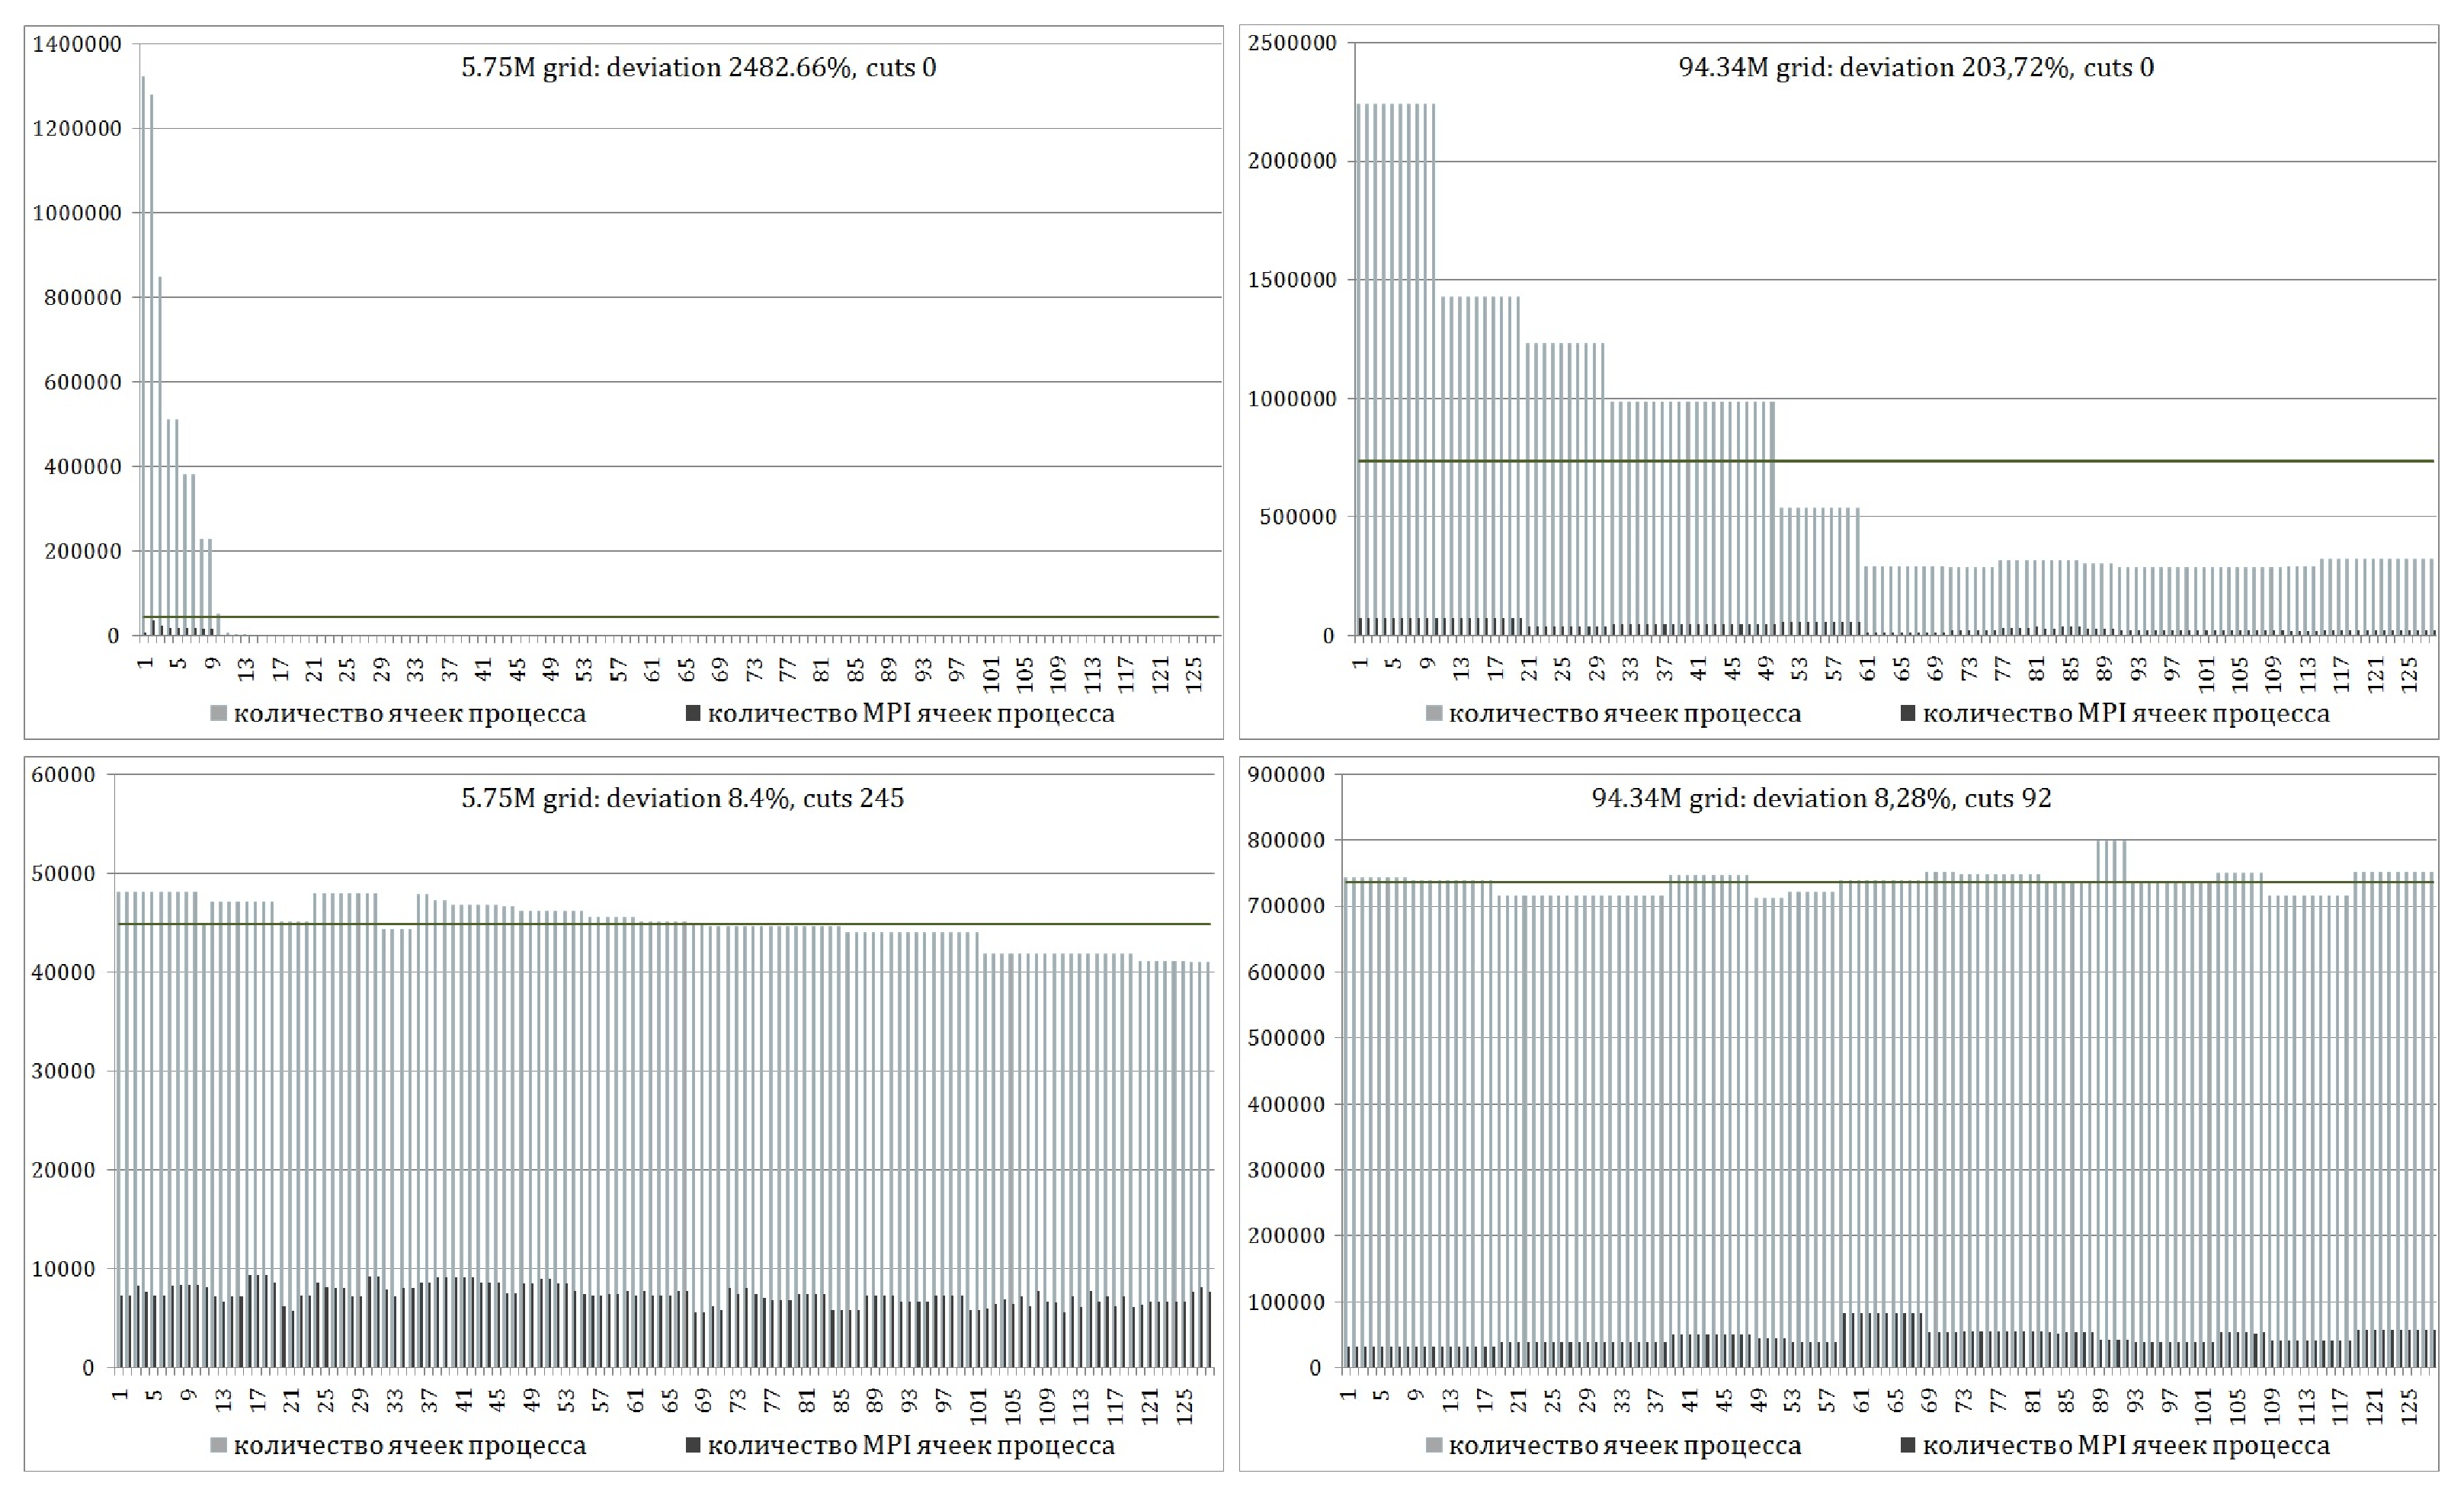
\includegraphics[width=1.0\textwidth]{./pics/text_2_withcut/withcut-charts.pdf}
\singlespacing
\captionstyle{center}\caption{Распределение блоков тестовых сеток (5,75 млн ячеек -- слева, 94,34 млн ячеек -- справа) без дробления (наверху) и с дроблением с допустимым отклонением $D^{\%} = 10\%$ (снизу).}
\label{fig:text_2_withcut_charts}
\end{figure}

Предложенный механизм распределения блоков блочно-структурированной сетки между узлами суперкомпьютерного кластера приводит к равномерной загрузке вычислительных ресурсов суперкомпьютерного кластера, что повышает эффективность его использования в расчетных задачах.
Часто применение такого подхода на большом количестве процессов приводит к кратному ускорению вычислений.
Особенно это актуально для сеток содержащих небольшое количество блоков или для сеток, имеющих ярко выраженные крупные блоки.

Негативным факторов применения дробления блоков является увеличение общего количества блоков и общего количества граничных ячеек, что приводит к увеличению объема данных межпроцессных обменов.

\subsubsection{Стратегии дробления блоков}

Рассмотрим различные стратегии дробления блоков при недостижении допустимого отклонения $D^{\%}$ при распределении блоков по процессам \cite{Bendersky2017Eff,Bendersky2018Block}.

Простейшая стратегия дробления блоков, использованная в предыдущем разделе, описывается следующим образом.
Сначала нужно применить жадный алгоритм распределения весов блоков по вычислительным узлам.
Если требуемое отклонение $D^{\%}$ наибольшего веса вычислительного узла от среднего значения достигнуто, то можно завершать работу.
В противном случае нужно разделить максимальный блок пополам по наиболее протяженному направлению, после чего произвести перераспределение.
Этот жадный алгоритм с дроблением пополам будем обозначать UG (от uniform greedy)\label{abbr:ug}.
Этот алгоритм всегда завершает работу, однако в отдельных случаях может выполнять необоснованно большое количество дроблений блоков, что приводит к возрастанию количества интерфейсных ячеек, а значит тормозит межпроцессные обмены между блоками сетки.

Для устранения крупных блоков без лишних дроблений предлагается механизм минимизации количества разрезов блоков.
Прежде всего определим, на какие части может быть разрезан конкретный блок, имеющий размеры $IS$, $JS$, $KS$ и содержащий соответственно $IS \times JS \times KS$ ячеек.

На возможные разрезы блока накладываются следующие ограничения.
Так как блок может быть разрезан только по границам ячеек, то размеры получившихся новых блоков будут кратны одному из значений $IS \times JS$, $IS \times KS$, или $JS \times KS$.
На самом деле, целесообразно выполнять разрезы только по наиболее протяженному направлению (пусть это будет $IS$, для каждого блока это направление будет свое), так как это приводит к минимизации количества интерфейсных ячеек.
Для запрета появления слишком тонких блоков по одному из измерений запрещается выполнять разрезы блока слишком близко к границе.
Для этого вводится специальный параметр $m$ (margin), по которому разрешается деление блока только в сегменте $[m, IS - m]$.
Вводится еще одно ограничение, не позволяющее производить слишком мелкие блоки (задается наименьшее допустимое количество ячеек в результирующем блоке, при котором разрешено дробление).

Алгоритм распределения блоков по вычислительным узлам с минимизацией количества разрезов (в дальнейшем будем обозначать его MCC, от minimal cuts count\label{abbr:mcc}) будем описывать в следующем виде:

1) Определить среднее ожидаемое количество ячеек, которое должно приходиться на один вычислительный узел, будем обозначать эту величину $mid$.
Она равна общему количеству ячеек сетки, деленному на количество вычислительных узлов $proc$.

2) Определить максимально допустимый вес вычислительно узла на текущий момент (будем обозначать через $max$).
Изначально $max$ берется равным $mid$.
Однако если в процессе распределения вес какого-либо вычислительного узла превысил $mid$, то величина $max$ принимает значение веса этого узла.
Таким образом $max$ определяется как максимум из величины $mid$ и всех весов вычислительных узлов.

3) Определить множество всех блоков, которые еще не распределены ни на один вычислительный узел.
Если это множество пусто, то алгоритм заканчивает работу.

4) Попробовать найти из рассматриваемого множества блоков такой блок, который можно распределить на один из вычислительных узлов так, чтобы вес этого узла не превысил $max$.
Если таких блоков несколько, то нужно взять такой блок, который максимально приближает вес соответствующего вычислительного узла к отметке $max$.
Если это удалось сделать, то распределить найденный блок на вычислительный узел и перейти к пункту 3.

5) Определить множество допустимых разрезов всех не распределенных на текущий момент блоков.
Каждый потенциальный разрез делит блок на две части.
Определить множество таких потенциальных результирующих блоков и из этих потенциальных блоков выбрать блок веса $w$ и вычислительный узел веса $W$ такие, что $W + w \le max$ и величина $max - (W + w)$ минимальна.
Если такой пары блок-узел не найдено, то найти такую пару, что $W + w > max$ и величина $(W + w) - max$ минимальна.
Такая пара найдется всегда.
После этого выполнить необходимый разрез для получения найденного блока и распределить его на соответствующий вычислительный узел, после чего перейти к пункту 2.

Кроме описанных действий приведенный алгоритм содержит ряд эвристик, не позволяющих проявляться негативным эффектам при возникновении сложных краевых случаев (например, неконтролируемый рост величины $max$). 
Таким образом, описанный  алгоритм на каждом шаге пытается выполнить такой разрез блока, чтобы максимально приблизить вес некоторого вычислительного узла к ожидаемой в среднем величине загрузки.

Для тестирования и оценки эффективности описанных выше методов распределения блоков блочно-структурированной сетки между узлами суперкомпьютерного кластера использовались три разные сетки, отличающиеся по количеству блоков: test (13 блоков, 5,8 млн ячеек), train (30 блоков, 10,7 млн ячеек), ref (136 блоков, 8,5 млн ячеек).

В качестве целевого вычислительного ресурса брался гомогенный вычислительный кластер\label{term:cluster_gomo2}, состоящий из 64 узлов.
Величина $m$, характеризующая минимальное расстояние разреза от границы блока, бралась равной 5.
На рис.~\ref{fig:text_2_withcut_2_merged_pic} представлены данные применения алгоритмов UG и MCC к каждой из приведенных расчетных сеток.
Описание данных на графиках: $mid$ -- средний ожидаемый вес вычислительного узла, $dev$ -- отклонение веса наиболее тяжелого узла от $mid$, $proc$ -- количество вычислительных узлов, $cuts$ -- количество выполненных разрезов, iface cells и cross cells -- доля интерфейсных и MPI ячеек среди всех ячеек сетки.

На каждом графике на рис.~\ref{fig:text_2_withcut_2_merged_pic}, представлена гистограмма распределения блоков расчетной сетки по вычислительным узлам.
Каждый столбец гистограммы соответствует одному вычислительному узлу.
Высота столбца -- вес соответствующего вычислительного узла.
Если к вычислительному узлу отнесены несколько блоков расчетной сетки, то соответствующий столбец гистограммы разделен на несколько частей, размеры которых отражают веса блоков, также эти части раскрашены в шахматном порядке для повышения наглядности.

\begin{figure}[ht]
\centering
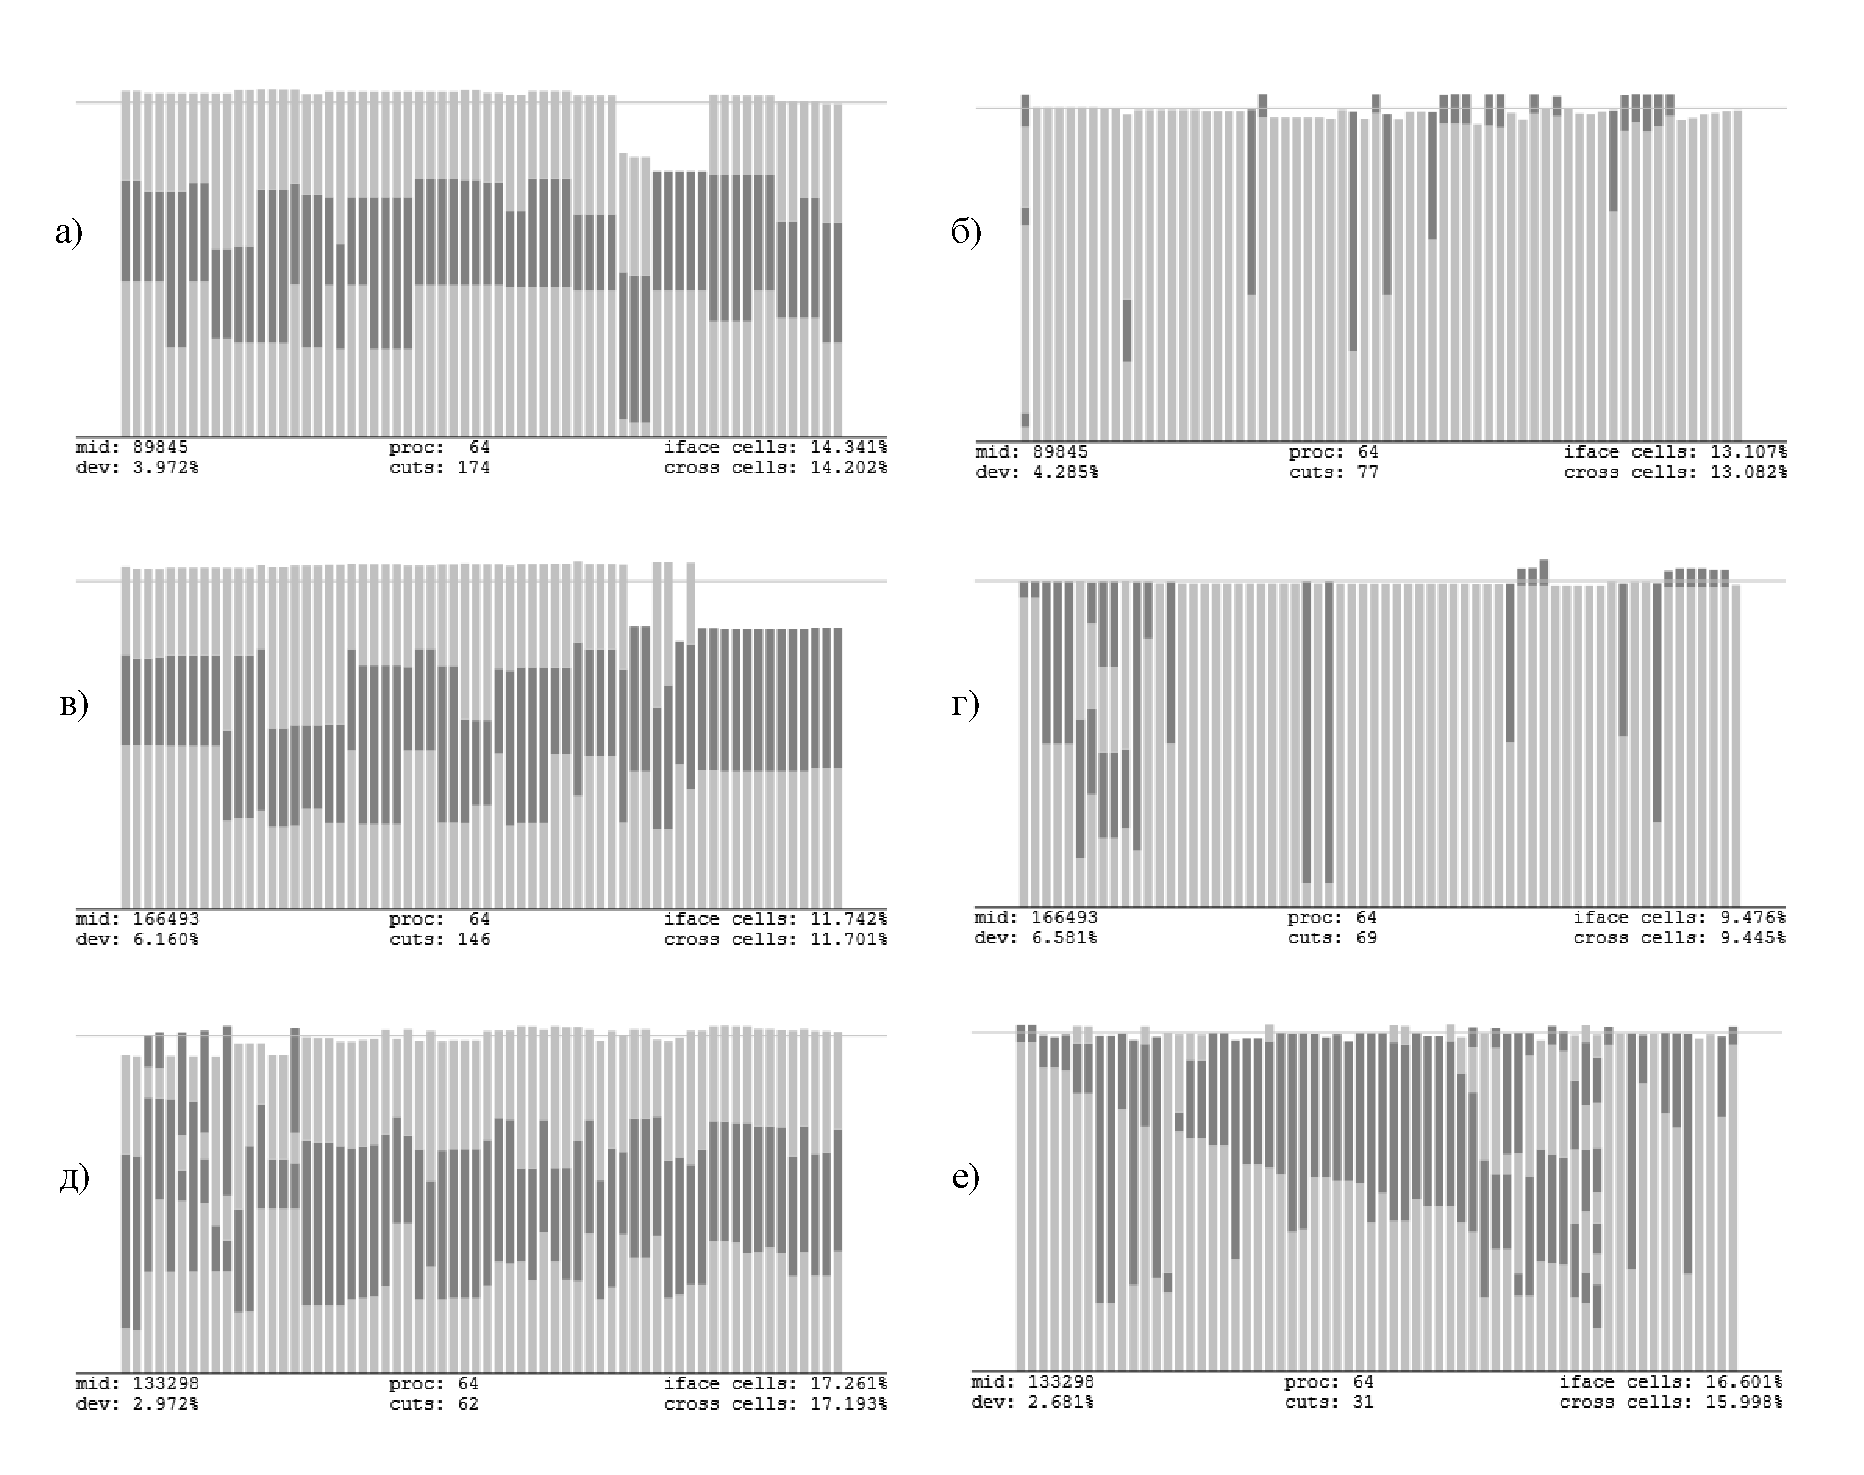
\includegraphics[width=1.0\textwidth]{./pics/text_2_withcut/2-merged-pic.pdf}
\singlespacing
\captionstyle{center}\caption{Гистограммы распределения блоков расчетной сетки по вычислительным узлам суперкомпьютера для сеток test (а, б), train (в, г), ref (д, е) с помощью алгоритмов UG (а, в, д) и MCC (б, г. е).}
\label{fig:text_2_withcut_2_merged_pic}
\end{figure}

Результаты сравнения эффективности методов UG и MCC распределения вычислительной нагрузки между узлами суперкомпьютера показывают, что использование метода MCC оправдано, так как с его помощью можно добиться распределения не худшего качества (а зачастую и лучшего), чем при использовании UG.
При этом MCC позволяет существенно сократить количество разрезов блоков сетки для достижения требуемого результата.
Также использование MCC приводит к сокращению количества MPI ячеек в сетке, что положительно сказывается на скорости межпроцессных обменов данными.
Особенно явно достоинства метода MCC проявляются на сетках с относительно небольшим количеством блоков и наличием ярко выраженных крупных блоков.

Для анализа эффективности метода распределения вычислительной нагрузки для блочно-структурированной сетки с дроблением узлов были произведены расчетны на модельном воздухозаборном устройстве высокоскоростного летательного аппарата, описанные в \cite{Bendersky2017Eff}.
Для этого объекта проводились численные расчеты на суперкомпьютере с использованием RANS/ILES метода.
Для проведения численных расчетов использовалась блочная расчетная сетка, содержащая 172 блока, 848 интерфейсов, 323 граничных условия, 12,8 миллионов ячеек.
Для распределения вычислительной нагрузки для этой сетки использовался алгоритм MCC с дроблением блоков.
В качестве вычислительного поля использовались узлы суперкомпьютера МВС-10П, каждый вычислительный узел содержит по 2 микропроцессора Intel Xeon E5-2697v3 (Haswell).
Были выполнены запуски расчетов в двух конфигурациях: с запуском двух MPI процессов на каждом процессоре и с запуском четырех MPI процессов на каждом процессоре.
Количество вычислительных узлов варьировалось от 1 до 18.
В качестве эталонного запуска, относительно которого считались ускорения, был выбран запуск на одном узле с двумя MPI процессами на каждом процессоре. 

\begin{figure}[ht]
\centering
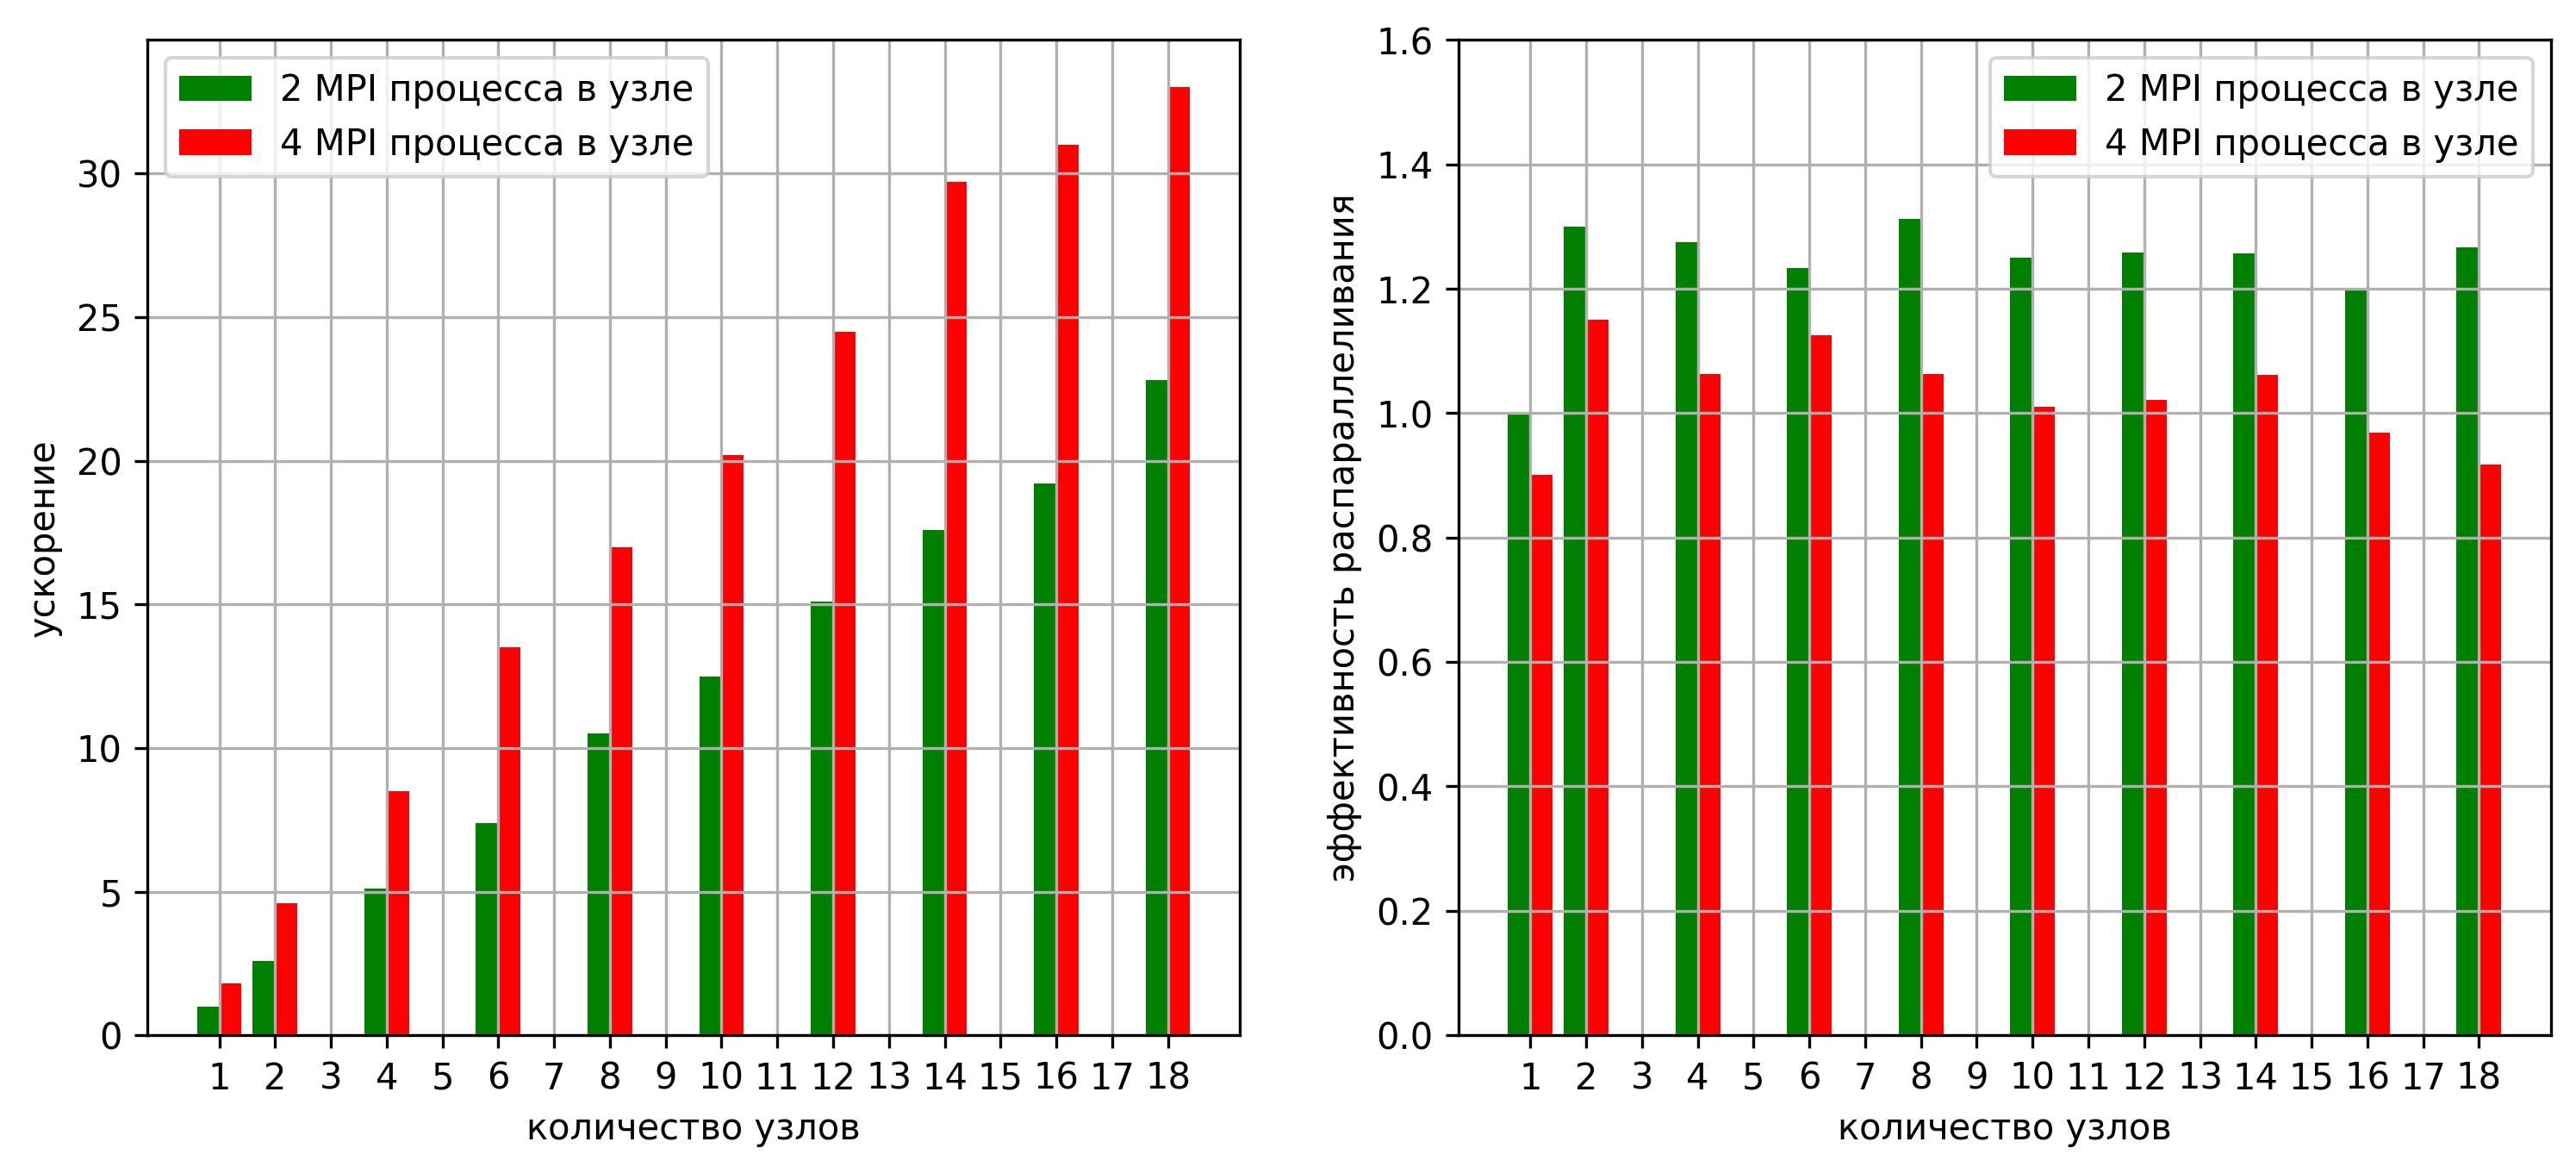
\includegraphics[width=1.0\textwidth]{./pics/text_2_withcut/scaling2.png}
\singlespacing
\captionstyle{center}\caption{Ускорение запусков и эффективность распараллеливания на различном числе узлов относительно эталонного запуска при проведении газодинамических расчетов на модельном входном устройстве воздухозаборника на суперкомпьютере с использованием RANS/ILES метода.}
\label{fig:text_2_withcut_scaling2}
\end{figure}

Из данных, приведенных на рис.~\ref{fig:text_2_withcut_scaling2}, можно видеть сверхлинейное ускорение при увеличении количества расчетных узлов.
Так, при использовании 18 узлов с двумя MPI процессами на каждом процессоре было достигнуто 23-хкратное ускорение относительно эталонного запуска.
Такое сверхлинейное ускорение объясняется как равномерностью распределения вычислительной нагрузки между узлами суперкомпьютерного кластера, так и снижением интенсивности и повышением локальности обращений в память при увеличении количества вычислительных узлов.
При использовании 4 MPI процессов на каждом процессоре эффективность счета увеличивается, при этом линейное масштабирование сохраняется.

\subsubsection{Масштабирование вычислений с разными порогами отклонения}

Для анализа эффективности распределения блоков по вычислительным процессам был поставлен эксперимент по выполнению численных  расчетов методом RANS/ILES на блочно-структурированной расчетной сетке, содержащей 9,4 млн ячеек \cite{Savin2019RANS}.

Перед вычислениями выполнялась подготовка расчетной сетки для 16, 32 и 64 процессов путем распределения вычислительной нагрузки с дроблением блоков сетки с помощью алгоритма UG, описанного в предыдущем разделе.
При подготовке расчетной сетки использовалось допустимое отклонение $D^{\%} = 10\%$, для подготовки вычислений на 64 процессах также использовалось допустимое отклонение $D^{\%} = 1\%$.

\begin{table}[!ht]
\centering
\singlespacing
\captionstyle{center}\caption{Характеристики используемых расчетных сеток.}
\bigskip
\label{tbl:text_2_withcut}
\begin{tabular}{ | l | c | c | c | c | }
  \hline
  Описание & Блоки & Интерфейсы & Граничые условия \\ \hline\hline
  360 градусов (94 млн ячеек) & 300 & 1796 & 1643 \\ \hline
  36 градусов (10,7 млн ячеек) & 30 & 152 & 204 \\ \hline\hline
  36 градусов, 16 проц., 10\% откл. & 39 & 224 & 218 \\ \hline
  36 градусов, 32 проц., 10\% откл. & 54 & 340 & 248 \\ \hline
  36 градусов, 64 проц., 10\% откл. & 170 & 982 & 429 \\ \hline\hline
  36 градусов, 64 проц., 1\% откл. & 383 & 2356 & 682 \\ \hline
\end{tabular}
\end{table}

\begin{figure}[ht]
\centering
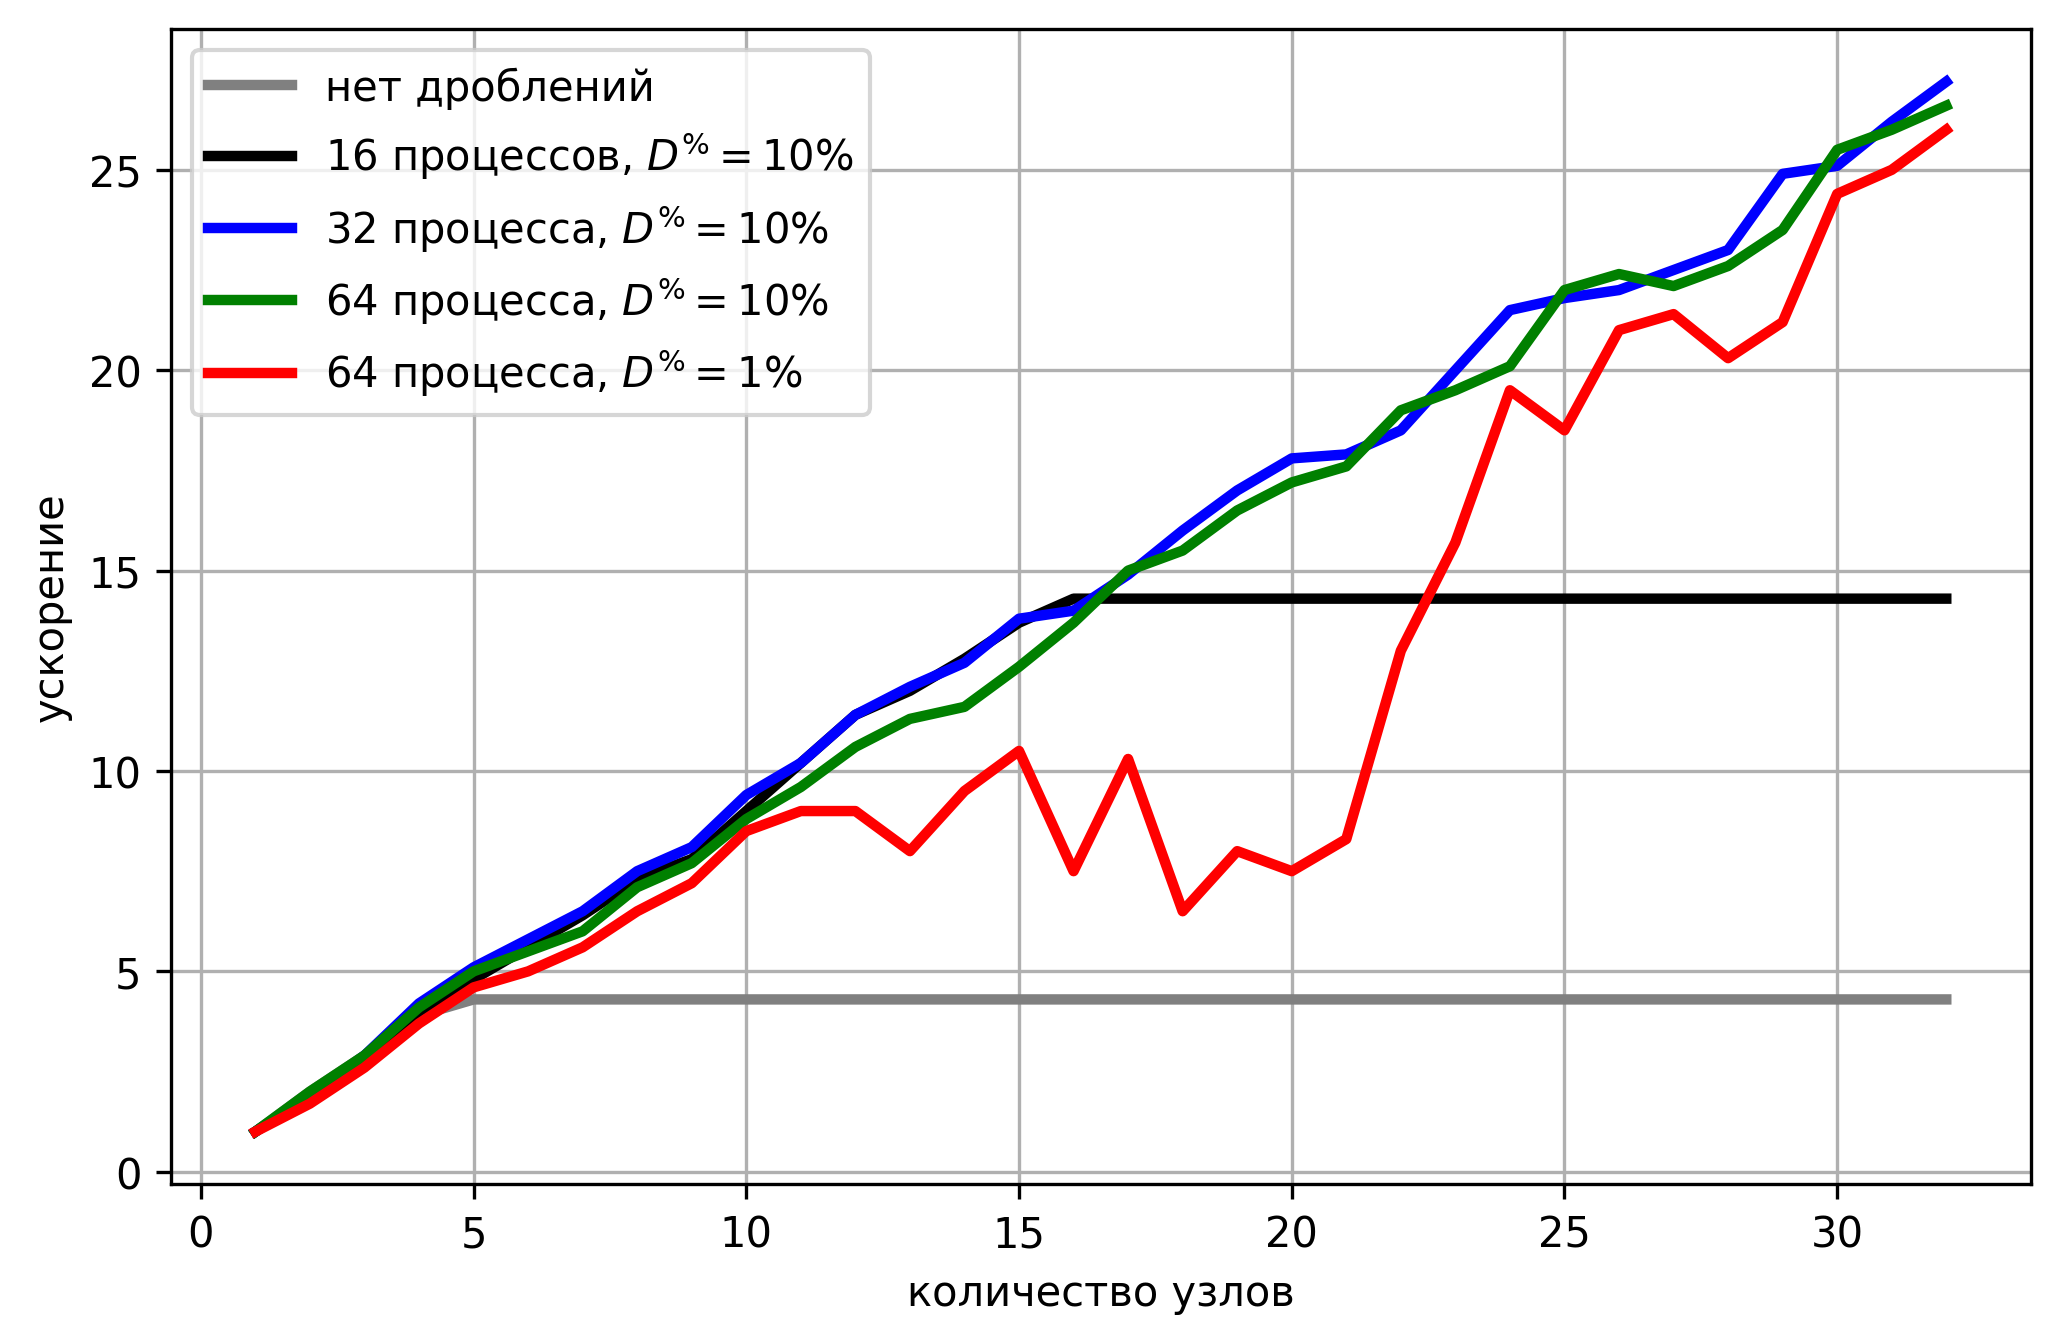
\includegraphics[width=1.0\textwidth]{./pics/text_2_withcut/scaling3.png}
\singlespacing
\captionstyle{center}\caption{Масштабирование вычислений при различных параметрах дробления сетки на 1-32 микропроцессорах Intel Xeon Phi Knights Landing 7290.}
\label{fig:text_2_withcut_scaling3}
\end{figure}

На рис.~\ref{fig:text_2_withcut_scaling3} представлены результаты численных экспериментов на сегменте суперкомпьютера МВС-10П, состоящем из узлов, каждый из которых содержит по одному микропроцессору Intel Xeon Phi Knights Landing 7290.
При проведении расчетов на каждом узле запускался один MPI процесс.
Количество узлов менялось от 1 до 32.
Проанализируем графики ускорения вычислений, представленные на рис.~\ref{fig:text_2_withcut_scaling3}.

Для вычислений на неподготовленной сетке (соответствует графику "нет дроблений") наблюдается ускорение для количества процессов до 5.
Далее ускорение остается на одной и той же отметке (около 4,3) и не меняется при дальнейшем увеличении количества узлов.
Это связано с наличием крупного блока, который мешает равномерному распределению вычислительной нагрузки.

При подготовке сетки для выполнения на 16 процессах (черный график) ускорение также останавливается, но на более высокой отметке (в районе 14,0).
Это также связано с наличием крупного блока, но его размер меньше, чем в случае отказа от дроблений (наиболее крупный блок был раздроблен, что привело к эффективному распределению вычислительной нагрузки для 16 процессов, однако для большего количества процессов размер этого блока препятствует равномерному распределению блоков по процессам).

При подготовке сетки для выполнения на 32 и 64 процессах с допустимым отклонением $D^{\%} = 10\%$ (синий и зеленый графики соответственно) получаем примерно одинаковое возрастание ускорения вычислений с ростом количества узлов.
Это говорит о том, что при подготовка сетки для большего количества процессов, чем реально будет использоваться для запусков, избыточно.

При подготовке сетки для выполнения на 64 процессах с допустимым отклонением $D^{\%} = 1\%$ (красный график) наблюдается сильная просадка по ускорению при использовании количества узлов от 10 до 25.
Это связано с сильным возрастанием количества MPI ячеек, что приводит к увеличению доли межпроцессных обменов.

Из графиков, приведенных на рис.~\ref{fig:text_2_withcut_scaling3}, можно сделать вывод, что при использовании распределения вычислительной нагрузки с дроблением блоков целесообразно предерживаться двух эвристических правил.
Во-первых, подготовку расчетной сетки не следует производить для количества процессов, больше того, которое реально будет использоваться при запусках.
Во-вторых, не стоит выбирать слишком низкий показатель допустимого отклонения $D^{\%}$, так как в случае слишком низкого значения этого показателя равномерность распределения вычислительной нагрузки будет нивелирована возрастанием объема межпроцессных обменов.
